\documentclass[11pt]{article}
\usepackage{amsmath, amssymb, amscd, amsthm, amsfonts}
\usepackage{graphicx}
\usepackage{hyperref}
\usepackage{tikz}
\usepackage{mathtools}
\usepackage{spverbatim}

% Korean packages
\usepackage[T1]{fontenc}
\usepackage{CJKutf8}

\oddsidemargin 0pt
\evensidemargin 0pt
\marginparwidth 40pt
\marginparsep 10pt
\topmargin -20pt
\headsep 10pt
\textheight 8.7in
\textwidth 6.65in
\linespread{1.2}

\title{Examining Algorithms to Win the game Rummikub\\
	\large MATH 818.01 Midterm Survey
}
\author{Jiyoon Jeong}
\date{}

\newtheorem{theorem}{Theorem}
\newtheorem{lemma}[theorem]{Lemma}
\newtheorem{conjecture}[theorem]{Conjecture}

\newcommand{\rr}{\mathbb{R}}

\newcommand{\al}{\alpha}
\DeclareMathOperator{\conv}{conv}
\DeclareMathOperator{\aff}{aff}

\begin{document}
	
	\maketitle
	
	\begin{abstract}
		This survey presents an overview of the possible algorithms that may be used to make an program that aims to win the board game, Rummikub. 
				
	\end{abstract}
	
	\section{Introduction}\label{section-introduction}
	
%	\begin{CJK}{UTF8}{mj}
%		한글 
%	\end{CJK}
	Rummikub is a number-based board game. The players do not know the tiles that other players have and strategies that they choose to play; that is, every player lacks information in the game theory during the game. Since there are 106 tiles and each player has only 14 tiles each initially, the player does not know which player has what tiles and what tiles are left. Besides, it is not necessary to give away every possible set on the board, so it is comparatively harder to predict other players' strategies or status than complete information game. Assume a situation that a player A has only finished one's initial meld but does not give away sets anymore and has comparatively many tiles like 23 tiles. That player may have no sets to put down but perhaps trying to complete as many sets as possible in advance. Due to the complex property of the game, devising a program that wins the game Rummikub is likely to require some special algorithm or approach. Before getting into that, this paper will cover case studiesthat solve or try to solve difficult but interesting games by using artificial intelligence (AI). Furthermore, the prior research of winning the game Rummikub in a way other than using AI will be covered as well.
	
		
%	\begin{theorem}[Helge Tverberg 1966 \cite{Tverberg:1966tb}]
%		Given $(r-1)(d+1)+1$ points in $\rr^d$, there is a partition of them into $r$ parts whose convex hulls intersect.
%	\end{theorem}
%	
%	\begin{figure}
%		\centerline{
\includegraphics[scale=1]{fig1-Tverberg}}
%		\caption{An example of a Tverberg partition.  The partition is not unique.}
%	\end{figure}
	
	%More formally, given $X\subset \rr^d$ of $(r-1)(d+1)+1$ points, there is a partition $X=X_1\cup \dots \cup X_r$ such that $\bigcap_{j=1}^r \conv X_j \ne \emptyset$. Such a partition is called a
	%\textit{Tverberg partition}. The number of points in this result is optimal, as a dimension-counting argument shows. In fact, if $X$ is in general enough position and in the partition $X=X_1\cup \ldots \cup X_r$ we have $1\le |X_j|\le d+1$ for every $j$, then $\bigcap_{j=1}^r \aff X_j$ is a single point if $|X|= (r-1)(d+1)+1$, and is empty if $|X|\le (r-1)(d+1)$.
	
	
	%The last decade has seen an impressive sequence of results around Tverberg's theorem.  The purpose of this survey is to give a broad overview of  the current state of the field and point out key open problems.  Other surveys covering different aspects of Tverberg's theorem can be found in \cite{Eckhoff:1979bi, Eck93survey, Matousek:2002td, BBZ17survey, de2017discrete, BZ17}.
	
	The paper is organized as follows:\\
	In section \ref{section-information} we introduce basic concepts prior to explaining the types of game in terms of complete information. Next, in the section \ref{section-alphago}, we describe case study of AlphaGo developed by Google Deepmind. In Section \ref{section-poker}, we describe what algorithms and learning were used to devise a Poker AI, Pluribus, to look over an example of incomplete information game AI. In Section \ref{section-ILP}, we introduce integer linear programming (ILP) to plan the Rummikub implementation using ILP in Section \ref{section-ILP imp}.
	
	
	%An early predecessor of Tverberg's theorem is Radon's lemma from 1921 \cite{Radon:1921vh, Eckhoff:1979bi}. Radon used it in his proof of Helly's theorem. It says that \textit{any set $X$ of $d+2$ points in $\rr^d$ can be split into two sets whose convex hulls intersect}. So it is the case $r=2$ of Tverberg's theorem. Its proof is simple: the $d+2$ vectors in $X$ have a nontrivial affine dependence $\sum_{x \in X}\al(x)x=0$ and  $\sum_{x \in X}\al(x)=0$. The sets $X_1=\{x \in X: \al(x)\ge 0\}$ and $X_2=\{x \in X: \al(x) < 0\}$ form a partition of $X$ and their convex hulls intersect, as one can easily check.
	
	
	%In a paper entitled ``On $3N$ points in a plane'' Birch~\cite{Birch:1959} proves that any $3N$ points in the plane determine $N$ triangles that have a point in common. His motivation was the (planar) centerpoint theorem. Actually, he proves more, namely the case $d=2$ of Tverberg's theorem and states the general case as a conjecture.
	
	%Tverberg's original motivation was also the centerpoint theorem and he learned about Birch's result and conjecture only later. He proved it first for $d=3$ in 1963, and in full generality in 1964.  Here is, in his own words, how he found the proof:  ``I recall that the weather was bitterly cold in Manchester. I awoke very early one morning shivering, as the electric heater in the hotel room had gone off, and I did not have an extra shilling to feed the meter. So, instead of falling back to sleep, I reviewed the problem once more, and then the solution dawned on me!'' \cite{tve:recollections}.
	
	
	%-----------------------------------------------------------------------------2
	\section{Complete and Incomplete Information Game}\label{section-information}
	There are diverse classifications of games. To name a few, zero-sum and non-zero-sum game, perfect and imperfect information game, and $n$-person game.
	To come up with algorithms to win the game Rummikub, it is meaningful to look over prior researches of similar kinds of games. 
	
	\subsection{Nash Equilibrium}
	
	A strategy is called a Nash equilibrium if no player can do better by unilaterally changing their strategy, assuming that each player knows others' strategy. In the example of the Prisoner's Dilemma, there is a dominant strategy: both confessing. Confessing is not always the best strategy, but it is the best strategy if `both' choose to confess. The Prisoner's Dilemma is described in the next subsection.

	\subsection{Utility Function}
	\textbf{Definition.}\\
	Utility function represents the degree of satisfaction of an input, which consists of various alternatives. Hence it reveals the preferences of the alternatives. The value of an output is to be maximized.
	
	
	From now on, we introduce the Prisoner's Dilemma in mathematical language.
		
	The set of players is $\{P_1, P_2\}$, $P_1, P_2$ distinct.
	
	The players are going to choose whether one will confess or deny, so there are two actions for each player, put it $A_1=\{C,D\}, A_2=\{C,D\}$ respectively. $C$ represents confession and $D$ represents denial.
	
	If both players choose to confess, then they each of them goes to prison for 3 years. If both choose to deny, then each of them goes to prison for 1 year each. If one confesses and the other denies, then the former goes free and the latter go to prison for 6 years. This is described on the table.
	
	The set of outcomes is $\{(C,C), (D,D), (C,D), (D,C)\}$.\\In one player's point of view, s/he does not know what the other player will choose but knows that the other player is offered the same deal as written below. Prisoner's Dilemma is an incomplete information game because the players do not know how the other player will act. Its definition is introduced in the next subsection.

\begin{center}
\begin{tabular}{cccll}
\cline{1-3}
\multicolumn{1}{|c|}{P1 / P2} & \multicolumn{1}{c|}{Confess} & \multicolumn{1}{c|}{Deny}    &  &  \\ \cline{1-3}
\multicolumn{1}{|c|}{Confess} & \multicolumn{1}{c|}{(-3,-3)} & \multicolumn{1}{c|}{(0,-6)}  &  &  \\ \cline{1-3}
\multicolumn{1}{|c|}{Deny}    & \multicolumn{1}{c|}{(-6,0)}  & \multicolumn{1}{c|}{(-1,-1)} &  &  \\ \cline{1-3}
\multicolumn{1}{l}{}          & \multicolumn{1}{l}{}         & \multicolumn{1}{l}{}         &  & 
\end{tabular}
\end{center}
	The utility of the player $P_i$ is $u_i(a_i, a_{-i})$ where $a_i$ denotes the action of a player $Pi$, and $a_{-i}$ denotes the action of the other player. Hence the result is as follows: 
	$u_i(C,C)=-3, u_i(D,D)=-1, u_i(C,D)=0, u_i(D,C)=-6$ $\forall i=1,2$.

%더 일반화된 정보는 여기에: http://classes.engr.oregonstate.edu/eecs/spring2019/cs331/slides/GameTheory1.2pp.pdf

	\subsection{Information Game}
	\textbf{Definition.}\\
	Information is literally the information that is or is not given to each player on the game.\\	
	\textbf{Definition.}\\
	Information is common knowledge if it is known to all the players, if each player knows that all the players know it, if each player knows that all the players know that all the players know it, and so forth ad infinitum. This is defined recursively.\\
	% Eric Rasmusen - An Introduction to Game Theory p47 
	%why defined recursively?
	\textbf{Definition.}\\
	Complete information game is a game where each player is fully aware of the rules of the game and the utility functions of every player.
	%Luce and Raiffa put it in their “Games and Decisions: Introduction and Critical Survey“, 1957,
	That is, each player has the common knowledge.
	
	%다른 해석
	If we look over the meaning of the concept `complete' itself, we can say as the following. Complete is a nature not moving first, or her initial move is observed by every player
	% Eric Rasmusen - An Introduction to Game Theory p48 명사 동사형만 좀 바꿈
	In a game of incomplete information, the meaning of complete is %that nature moves first and is unobserved by at least one of the players. Otherwise the game is one of incomplete information.
	% p50
	In contrast, an incomplete information refers to situations where some of the elements of the game are not common knowledge.
	The game Rummikub is classified into an incomplete information game which is an opposite concept of a complete information game.
	
	
	The concepts explained so far can also be demonstrated in mathematical language and this is dealt in many books of Game Theory, as such, reference~~%여기 표시
	Perfect is also a popular concept when classifying the game because it is the strongest informational requirement. To put it another way, every player knows the meaning and strategies of other players' play. Besides, incomplete games are also imperfect games. The game Go, Chess and Shogi which are played smartly by AlphaZero are all perfect information games. Starcrafts2 and Poker are imperfect information games.
	
	%-----------------------------------------------------------------------------3
	\section{Case Study: AlphaGo}\label{section-alphago}
	As seen in Section \ref{section-information}, the game of Go is a complete information game. AlphaGo is consists of Deep Neural Network (DNN) and Monte Carlo Tree Search (MCTS). In this survey paper, we only go through MCTS.
	
	List of the methods is as follows: Supervised Learning (SL) of policy network, Reinforcement Learning (RL) of policy network, RL of value network, Searching with policy/value network (which is MCTS).
	%논문 목차 따온 것임
	
	DNN is trained by humans and by itself to make AlphaGo a smarter player and MCTS efficiently searches the best move to choose it. Policy network and value network are improved by the training process of DNN and rollouts--playouts or single game from the beginning to the end--are made to update winning scores of nodes in search tree.

	The policy network chooses the best next move. Move changes the current state by choosing an action, and turn it into the next state. Both SL and RL are used to improve policy network--that is, to make policy network smarter hence it can choose the best move. SL learns strategies given by human experts while RL is learned by self-plays.
	% Medium A brief introductino ~ 참고	 policy 에 대한 정의도 해야하나?
	
	Value network calculates the probability of final win when the move is suggested by policy network.
	
	Rollouts are done randomly as the third step of Monte Carlo simulations.
	%diagram?
	
	
	\subsection{Monte Carlo Tree Search (MCTS)}

	\textbf{1. Monte Carlo Method}\\	
	This method is done in heuristic way, that is, it is empirical method using probability. 
	%MC is used in Mathematics and Physics; simulations of the Manhattan Project and invention of a hydrogen bomb, to name a few. 
	The phenomenon of neutron collision is the background of this method%and is also the principle of devastating atomic bomb
	. The neutrons collide with one another, splits apart, thereby expelling neutrons. Here, splitting is occurred under the conditions of certain probabilities so these probabilities should be clearly known. The whole process is iterated and dispersed, hence leads to inducing explosion.

% 이건 발표 때? 수학자 폰 노이먼과 노벨물리학상을 받은 페르미(Fermi) 등은 시뮬레이션을 통한 통계적인 방법만이 이 확률을 계산할 수 있다는 결론을내렸다. 전산기가 아직 개발되지 않았던 때였고 이 시뮬레이션을 위해절반은 전기적,절반은 기계적인 기구를 개발하여 사용했다. 이 확률 계산에 몬테카를로 방법이란 이름이 붙었는데 아마도 중성자들의 무작위충돌 분열 현상이 도박과 비슷하고, 몬테카를로가 도박의 대명사였기 때문이라 생각한다. 혹자는 이 프로젝트의 일원으로 실용 가능한 폭탄설계를 한 수학자가 포커광이어서 도박에 관계된 이름을 지었다고도 한다.
	The mainstream of this algorithm is the idea that even a deterministic mathematical problem can be solved in a heuristic method using random sampling. The procedure is as follows: generating random number and calculating probability of certain goal information by using random number. As the number of iteration goes to infinity--in reality, the number increases--, the output value gets closer to the goal information--for example, winning scores of certain path.
	
	Simple examples are computing $\pi$, ratio of the circumference of a circle to its diameter and the Buffon Needle problem. The code of the first example is attached in this page. Think of a square with a side length of $1$ and the circle inscribed in the square. Each area of a figure is $1$ and $\frac{\pi}{4}$ respectively. Then we calculate the probability of the points that goes inside the circle. If there are sufficiently many points, then we can estimate that (the probability of the points in the circle) $\times 4 \approx \pi$. The code is written in python language.
	\begin{spverbatim}
	import random
    
x = 0
y = 0
circle = 0
count = 0

while True:
    for i in range(0, 1000000):
        x = random.random()
        y = random.random()
           
        if (x * x) + (y * y) <= 1:
            circle += 1
            
        count += 1

    print(count, (circle/count) * 4, sep=": ")

	\end{spverbatim}\\
	
	The result is as follows: \\
	\textbf{2. Monte Carlo Tree Search}\\
The goal of this algorithm is to predict winning rates of paths of nodes without going through every single path. These days, MCTS is treated as a basic and prioritized searching algorithm after it was used in AlphaGo.\\

\begin{figure}
  \centering
  \includegraphics[width=\linewidth]{MCTS_pic1.jpg}
  \caption{The diagram describing the process of MCTS}
  \label{fig:MCTSdia}
\end{figure}

The process is as follows:\\


	1) selection: 
	In the selection phase, the algorithm starts at the root node and chooses a child node that has the maximum win rate at each node. It only extends to one further depth. The evaluation is done by Upper Confidence Bound applied to trees (UCT) formula:
\begin{equation}
\begin{aligned}
	UCT_i = \frac{w_i}{n_i}+c\sqrt{\frac{\ln{t}}{n_i}}, where\\
	w_i = \text{number of wins after the i-th move,}\\
	n_i = \text{number of rollouts after the i-th move,}\\
	c_i = \text{exploration parameter and }c_1= \sqrt{2},\\
	t = \text{total number of simulations for the parent node,}\\
\end{aligned}
\end{equation}
	
	The first term means the win rate and represents the exploitation and the second term exploration; we can see exploit-explore tradeoff in this formula. The former value is relatively higher value for moves with high average win rates. On the other hand, the latter value is higher for moves that undergone few simulations. %대충 값 얼마나 나오지?\\
The meaning of the second term...
	The UCT is theoretically proven to converge to MiniMax search, but practically, basic version of MCTS converges to MC Perfect game, which is not as thorough as MiniMax search.\\
	MiniMax searching goes through every single node. If the implementation time takes too long, then traversal is gone through so far as the nodes in the certain depth. If this happens, then the result of the algorithm becomes far from the intended result.

	
	2) expansion:
	In the expansion phase, one child node is expanded from the selected node. 	
	
	3) simulation: In the simulation phase, simulation is the random rollout starting from the child node expanded in the former state which is generated by RL.
	
	4) update(backpropagation): In the update phase, the algorithm goes back along the path to update the visit score and winning score of each node (or game state), thereby changing the UCT function. In this way, the node selection in the next round will be closer to win rates of winning tactics if they exist.\\
	\\
	\textbf{3. Advantages and disadvantages of MCTS}\\
1) Advantages: \\%성능이 실질적으로 얼만큼 좋아지는지.. 10^380 짜리는 minimax 로 안되고 deep blue 는 이걸로 체스 (10^123) 이겼었다
2) Disadvantages: Aside from the issues of a huge amount of memory and a speed. If the machine encounters unusual situation, then it chooses absurd decision. Since the search cannot cover every single case but covers only paths with the high win rate, some paths are gone through insufficiently. This phenomenon was shown in Game four of AlphaGo versus Lee Sedol (or the Google DeepMind Challenge Match). It is interpreted that Lee's unexpected play at white 78 would have made AlphaGo's poor respond on move 79, leading to Lee's win.\\

	code for tic-tac-toe (only MCTS)



%	\begin{CJK}
%	
%	
%	처음에 score 들은 다 0 에서 시작(근데 그러면 첫 게임할 때는 어떻게 가지?) 게임을 한 번 끝까지 할 때마다 score 이 업데이트 돼어 iteration 이 많이 진행되면 점점 데이터가 쌓여서 승리하는 path(moves) 의 score 이 높아지도록 수렴한다(수렴한다는 말이 너무 무책임하네.. 구체적으로 어떻게, 어떤 식으로 수렴?).
%	
%	게임이 끝난 상태에서 왜 expansion을 한다는 거야?
%	
%	\end{CJK}
	
	
	
	
	
	
	Alphazero also used MCTS to average the approximation errors made by non-linear function approximation, not alpha-beta pruning.
	
	\subsection{Alpha-beta Pruning}
	%설명하고 propagates the biggest approx erros ....
	
	Alpha-beta pruning is a kind of search algorithm to cut down unnecessarily leaves as far as they do not affect the result. It is a kind of MiniMax searching.Alpha-beta search computes an explicit MiniMax, which propagates the biggest approximation errors to the root of the subtree. It requires a function to evaluate current state in every step, hence needs a great deal of computation of levels in the game tree to find the optimal move.
	
	%이유는 모르겠으나 alpha-beta pruning 이 더 error 컸다. MCTS 가 더 error 작다.
	
	%searching algorithm usually reduces the computational space 
	
	
	%-----------------------------------------------------------------------------4
	\section{Poker AI}\label{section-poker}
	
	Poker is one of the most popular games that have a property of incomplete information. Many researchers strives to devise an AI that solves the Poker. There were several AIs of such, and one of them, Pluribus, is superhuman AI for multiplayer poker. DeepStack is AI of 2-player.
	
	
	DeepStack uses the following algorithms.
		
	Pluribus was shown to be stronger than top human experts in six-player no-limit Texas hold'em poker. In most cases to solve a game problem, finding Nash equilibrium is the usual goal. However, in this case, it is theoretically hard to find Nash equilibrium, so the researchers focused on finding solutions in empirical means.\\
	
	Things to consider: \\
	1. As the number of players grow, it is computationally almost impossible to solve the game to the end.\\
	2. A player's optimal strategy for a particular situation changes as other players' strategy is for every situation. 

	Used algorithms:\\
	Pluribus is learned by only self-plays, without any prior data or strategies given. There are $3$ representative methods and two of them are deep-limited searches.\\	%what is deep-limited searches
	First is the blueprint strategy computed using Monte Carlo counterfactual regret minimization (MCCFR) and Linear CFR. CFR is an iterative self-play algorithm that starts with random play to beat earlier versions of itself.\\ %p3
	Second is real-time search. Real-time search is necessarily used in solving complete information game. MCCFR is used when the scale of computation is relatively small, but an optimized vector-based form of Linear CFR is used otherwise.\\
	
	
	Abstraction is used to make the calculations scalable before applying the above strategies. 
	Action abstraction reduces the number of actions. Here, making bet is an action, so only some selected bet sizes are used. If it becomes off-tree search, the algorithm finds the most similar target--that is, size.\\
	Information abstraction reduces the number of situations. Consequently, it drastically reduces the complexity of the game.
	%그래서 어디다가 사용한다는 말인가?
%	\textbf{Definition.}\\
%	Blueprint strategy
	%Pluribus's self-play produces a strategy for the entire game offline, which we refer to as the blueprint strategy.
	Pluribus runs on a relatively small capacity of CPUs and memory. AlphaGo used 1920 CPUs and 280 GPUs for real-time search in 2016, but Pluribus used two Intel Haswell E5-2695 and uses less than 128 GB of memory.
	
	
	%-----------------------------------------------------------------------------5
	\section{Integer Linear Programming}\label{section-ILP}
	
	Linear Programming (LP), or linear optimization, is an optimization problem in which the objective function is linear in the unknowns and the constraints consist of linear equalities and linear inequalities. LP is not a computer-based implementation, but only a mathematical method. For example, the simplex method is founded on the fact that the optimal value of a linear programis finite, is always attained at a basic feasible solution. %ref Linear and Nonlinear Programming 3rd ed David G. Luenberger 파란 책p70
	
	Optimization includes maximizing or minimizing a linear functional over a set of constraint polynomials. Linear equations can be reduced to a vector and matrix notation.


	$\bf{A}$ is an $m \times n$ matrix, $\bf{x}, \bf{c} \in \mathbb{R}^{n}$, $\bf{b} \in \mathbb{R}^{m}$ 

\begin{equation}
\begin{aligned}
	\text{minimize } &\bf{c}^{T}\bf{x}\\
	\text{subject to } &\bf{Ax} = \bf{b} \text{ and } \bf{x} \geq 0.
\end{aligned}
\end{equation}
	
	%\begin{theorem}[Fundamental theorem of linear programming] %\cite{} ] 안쪽에
	%	Given a linear program in standard form $(1)$ where $\bf{A}$ is an $m \times n$ matrix of rank $m$,\\
	%	{i)} if there is a feasible solution, there is a basic feasible solution;\\
	%	{ii)} if there is an optimal feasible solution, there is an optimal basic feasible solution.	
	%\end{theorem}

	%The theorem states that 
	
	
	Integer linear programming is a linear programming whose every entry of solution vector is integer.
	
	
	Maximize the value of $y - \frac{1}{x}$ on the region surrounded by $x \geq 0, y \geq 0, y \leq -0.9 x + 2.4$
	
	\begin{center}
	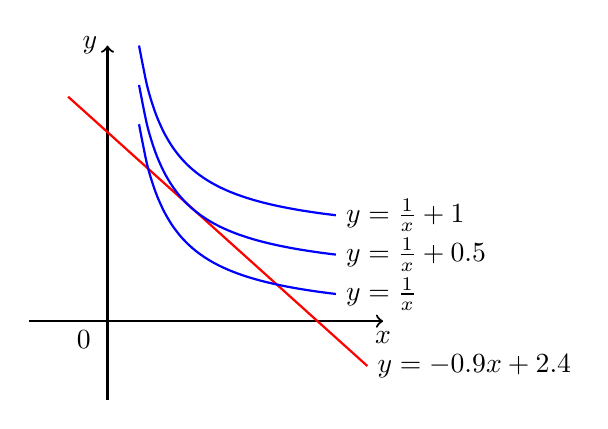
\begin{tikzpicture}[scale=1]
	
	\draw [thick, ->] (-1,0) -- (3.5, 0) node [anchor = north] {$x$};
	\draw [thick, ->] (0,-1) -- (0,3.5) node [anchor=east] {$y$};
	
	\node [below] at (-0.3,0) {$0$};
	\draw[domain=-0.5:3.3, smooth, thick, , variable = \x, red, text=black] plot ({\x}, {-0.9*\x+2.4}) node[right]{$y=-0.9x+2.4$};
	\draw[domain=0.4:2.9, smooth, thick, , variable = \x, blue, text=black] plot ({\x}, {1/(\x)}) node[right]{$y=\frac{1}{x}$};
	\draw[domain=0.4:2.9, smooth, thick, , variable = \x, blue, text=black] plot ({\x}, {1/(\x)+1}) node[right]{$y=\frac{1}{x}+1$};
	\draw[domain=0.4:2.9, smooth, thick, , variable = \x, blue,text=black] plot ({\x}, {1/(\x)+0.5}) node[right]{$y=\frac{1}{x}+0.5$};
	\end{tikzpicture}
	\end{center}
		
	Put $k=y - \frac{1}{x}$.
	
	$y=\frac{1}{x}+k$ has the form of graph as illustrated as blue graphs. The graph should satisfy the following conditions: it should be on the region--some point on the graph should also be on the region--and it should make $k$ maximum. Combining these two conditions, we can conclude that the graph should be as high as possible starting from $x$-axis, still meeting the region. Since $y = \frac{1}{x}+k$ has derivative $y' = -\frac{1}{x^2}$ on $(0,\infty)$, we can conclude that there exists some $(x,y)$ such that $y' = -0.9$. That is, there exists $k$ such that $y = \frac{1}{x} + k$ tangent to $y=-0.9x +2.4$. By calculations, two graphs meet tangentially at the point $(\frac{1}{3}\sqrt{10}, -\frac{3}{10}\sqrt{10}+2.4)$. By putting this value into $y = \frac{1}{x} +k$, we get the maximum $k=-\frac{3}{5}\sqrt{10}+2.4$
	
	
	We will see specific implementation of ILP in Section \ref{section-ILP imp}.
	
	
	
	%-----------------------------------------------------------------------------6
	\section{Basic rules of the game Rummikub}\label{section-rules}
	
	There are total 106 tiles--2 sets of tiles numbered 1 to 13 in four colors: black, red, blue, orange; 2 Jokers. There are 4 racks that the players can put their tiles on, hence 2 to 4 players can join the game.
	meld
	A set is ~
	Each players has a turn and when it is one's turn, that player give out sets or 
	A group is a set of either three or four tiles of the same number in different colors.
	A run is a set of three or more consecutive numbers, all in the same color.
	
	\textbf{Scoring system}
	
	The game is finished when there is a player who has no tile left.
	The winner is determined by the score in the highest order: the player who first finished the rack wins and gets the score after calculating the scores of the others. Each player's score is the negative sum of the values of the tiles left. The winner's score is the sum of each player's sum of values of the tiles, which is positive. The Joker tile is counted as the value of $50$ if it is on the rack. If the player did not completed the initial meld, then the score is $-100$.
	
	
	%-----------------------------------------------------------------------------7
	\section{ILP on Rummikub}\label{section-ILP imp}
	
	There are two goals of this programming:\\
	(1) The major goal is to maximize the value of the tiles that can be placed onto the table.\\
	(2) The minor goal is to minimize the movements of the existing sets on the table.\\
	It seems like this programming is a greedy algorithm if we only look over the major goal. However, in order to consider real practice, changing as small sets on the table as possible is more efficient in terms of time, energy, and memory like a human.\\
	
	First, give the model:
	
	\textbf{Indices ($I$, $J$ are mathematical sets)}\\
	$i \in I$ indicates the type of the tile (defined by color and number), $I=\{1,2, \cdots , 53\}$\\
	$j \in J$ indicates the index of the set (run or group), $J=\{1,2, \cdots, 1174\}$\\
	
	There are $2$ copies of $13\times4=52$ tiles with $2$ Jokers whose roles are indistinguishable. Hence there are $53$ types of tiles. That explains the index set $I$.
	
	To explain $J$, the number of Jokers should be taken into account.\\
	
	
\begin{tabular}{|c|r|r|r|c}
\cline{1-4}
Number of Jokers & \multicolumn{1}{c|}{0} & \multicolumn{1}{c|}{1}       & \multicolumn{1}{c|}{2}           & Total \\ \cline{1-4}
groups of $3$    & $13\times4=52$         & $13\times{{4}\choose{2}}=78$ & $13\times4=52$                   & 182    \\ \cline{1-4}
groups of $4$    & $13$                   & $13\times{{4}\choose{3}}=52$ & $13\times{{4}\choose{2}}=78$     & 143   \\ \cline{1-4}
runs of $3$      & $11\times4=44$         & $(12+11)\times4=92$          & same case as 'groups of $3$' & 136   \\ \cline{1-4}
runs of $4$      & $10\times4=40$         & $(11+10+10)\times4=124$      & $(12+11+10)\times4=132$          & 296   \\ \cline{1-4}
runs of $5$      & $9\times4=36$          & $(10+9+9+9)\times4=148$      & $=233$                           & 417   \\ \cline{1-4}
\end{tabular}\\


Total number of sets is 1174\\
\\
%왜 233 나왔지
{\large 1) The linear programming only reflects goal (1)}

	\textbf{Parameters}\\
	$s_{ij}$ indicates whether tile $i$ is in set $j$ (yes$=1$, no$=0$),\\
	$t_j$ indicates the tile $i$ is $0,1$ or $2$ times on the table,\\
	$r_j$ indicates the tile $i$ is $0,1$ or $2$ times on your rack.
	
	
	\textbf{Variables}\\
	$x_j$ indicates that the set $j$ can be placed $0,1$ or $2$ times onto the table,\\
	$y_i$ indicates that the tile $i$ can be placed $0,1$ or $2$ from rack onto the table.

	
	\textbf{Objective and constraints}\\
\begin{equation}
\begin{aligned}
	\max\sum_{j=1}^{53}v_iy_i
\end{aligned}
\end{equation}

	
	
	subject to
	
	\[\sum_{j=1}^{1174}s_{ji}x_j=t_i+y_i\text{ } \forall i\]
	\[y_i\leq r_i\text{ } \forall i\]
	\[x_j\in\{0,1,2\}\text{ } \forall j\]
	\[y_i\in\{0,1,2\}\text{ } \forall i\]

	The meaning of the constraint is.. %??
	
	
	This model contains at most 1174 variables and 53 real constraints. Furthermore, note that this model is always feasible: ....\\
%	\textbf{Definition.}\\
%	A vector $\bf{x}$ satisfying some constraints is said to be feasible for these constraints. In other words, we can say that a solution that satisfies the constraints is called a feasible solution.
\\%구조통일 조심
{\large 2) The next linear programming given includes goals (1) and (2).}
	
	
	\textbf{Parameters}\\
	$w_j$ set j is $0,1$ or $2$ times on the table\\
	$M$ constant (a number more than 35, default 40)
	
	\textbf{Variables}\\
	$z_j$ the difference between the number of occurrence of the set $j$ in the new solution and the old solution.
		
	
	\textbf{Objective and constraints}\\
\begin{equation}
\begin{aligned}
	\max\sum_{j=1}^{53}v_iy_i+\frac{1}{M}\sum_{j=1}^{1174}z_i
\end{aligned}
\end{equation}

	subject to
	
	\[\sum_{j=1}^{1174}s_{ji}x_j=t_i+y_i\text{ } \forall i\]
	\[y_i\leq r_i\text{ } \forall i\]
	\[z_i\leq x_i\text{ } \forall i\]
	\[z_i\leq w_i\text{ } \forall i\]

	\[x_j\in\{0,1,2\}\text{ } \forall j\]
	\[y_i\in\{0,1,2\}\text{ } \forall i\]
	\[z_i\in\{0,1,2\}\text{ } \forall i\]
	
	If we only consider the condition (1), $\max\sum_{i=1}^{53}v_iy_i$ in which $v_i$ is the value of the tile $i$.
	
	
	%문제 해설
	%식 해석
	%
	
	
	There are at most $35 = \lfloor \frac{53\times2}{3} \rfloor$, because there are $106$ tiles and the shortest possible length of a set is $3$. 
	
	
	
	
	The ILP model is implemented in AIMMS (Advanced Integrated Multi-Dimensional Modelling Software) on a Pentium \uppercase\expandafter{\romannumeral3}
	
	

	%anyone can do until now



%	\section{ILP on My First Rummikub}\label{section-ILP MFR}
%
%	이걸 직접 할 수 있는지 알아보기. 식은 변형만 하면 됨.


	%-----------------------------------------------------------------------------8
	\section{Planning Implementation}\label{section-imp}
	
	
	%아니면 어떤 걸 써야할 것 같은지에 대해 쓰고 implementation 은 기말 과제로!
	There are $4$ goals of this programming:\\
	(1) The major goal is to maximize the number of value of the tiles that can be placed onto the table.\\
	(2) Another minor goal is to prioritize two numbers $13,12,1,2$ in this order.\\
	(3) Use the Joker only if there is no other set.\\ % 근데 joker 는 안 내면 마지막에 가장 크게 점수 까이는데 어쩌징.
	(4) One minor goal is to minimize the movement of the existing sets on the table.\\

	
	From now on, the reasons why such goals were suggested be explained intuitively with examples.
	
	
	To explain (2), intuitively, the number $13,1$ and $12,2$ have comparatively less possibility to form a set and since their values are among the highest, these numbers should be put down as soon as possible. We cannot calculate every single case of certain set being on the table in advance. Hence we only briefly consider the probability of being part of a set as follows:\\
	$13,1$: $\frac{}{1174}$
	$12,2$: $\frac{}{1174}$
	%솔직히 진짜 1174인지도 모르겠음
	
	
	To explain (3), even if using the Joker tiles is the only way, a human player does not necessarily put down one's set. The player may wait until suitable sets appear without using the Joker tiles. The strategy depends on the player, but (1) contradicts with the strategy to make the best use of the Joker tile; that is, to use the Joker in the 'best' situation. For example, assume that the player A has the tile (mathematical) set $\{2(black),4(black),7(orange),8(orange),Joker \}$. According to this program, using the Joker is the only way to put down the set. $\{7(orange), 8(orange), Joker\}$ or $\{Joker,7(orange), 8(orange) \}$, $\{2(black), Joker, 4(black) \}$ are the only ways. However, a human player may be looking forward to obtain $3(black), 6(orange), 9(orange)$ in one's turn because the possibility to complete the runs is not very low compared to the situations like below.
	
	
	However, assume this case: $\{1(black),5(black),7(orange),8(orange),Joker \}$. How would a player act? In order to reduce the total value of the rack, the player would probably follow the goals suggested above. Or, others would choose to obtain new tiles to complete black tiles--1,2,3,4,5--or orange tiles--6,7,8 or 7,8,9. There is a big assumption to consider: the present state. What if there are already some tiles on the board? What if those tiles are not to be utilized; that is, unchangable in the present status?
	
	
	Hence, it is very hard to make all situations into consideration.
	
	
	In my personal point of view the minor goal suggested by the previous section is a lot more minor than the other goals suggested above. Since it has value less than value of any tile, its weight is very low. Hence we use the second term of the formula $(2)$
	%계산하는 시간이나 두는 시간이 제한시간보다 길지는 않을 것 60초 정도인데.. 이걸 어떻게 설명하지. 근거는?
	
	(4) One minor goal is to minimize the movement of the existing sets on the table.\\
	%이걸 다 수학적으로 어떻게 하지??	
	
	Computer of a high capacity is (or are) needed in order to implement this ILP.
	
	\bibliographystyle{alpha}
	\bibliography{references} % see references.bib for bibliography management
	
\end{document}


% 필승패 있는지.. 